% \documentclass[prb,showpacs,amsmath,amssymb,twocolumn]{revtex4}
% 
% \usepackage{dcolumn}
% \usepackage{verbatim}
% \usepackage{graphicx}
% \usepackage{epsfig} % multi-line comments
% \usepackage{hyperref}
% 
% \begin{document}
% \newcommand{\boldnabla}{\mbox{\boldmath$\nabla$}}
% 
\chapter{2D THUE-MORSE ARRAY OF OPTICAL CAVITIES: TIGHT-BINDING MODEL}
\label{eq:TM_physics}
\label{paper:6_start}

% 
\begin{center}
Ben Payne$^1$, Laura Sisken$^1$, Heeso Noh$^2$, Hui Cao$^2$, Alexey Yamilov$^1$                                                                               \end{center}

\ \\
% \author{Ben Payne$^1$, Laura Sisken$^1$, Heeso Noh$^2$, Hui Cao$^2$, Alexey Yamilov$^1$ \footnote{Electronic~address:~yamilov@mst.edu}}
\begin{center}
\textit{$^1$Department of Physics, Missouri University of Science \& Technology,\\ Rolla, MO 65409\\
$^2$Department of Applied Physics, Yale University, New Haven, CT 06520}\end{center}

\ \\
% \affiliation{$^1$Department of Physics, Missouri University of Science \& Technology, Rolla, MO 65409\\
% $^2$Department of Applied Physics, Yale University, New Haven, CT 06520}
% 
% \date{\today}
% 
% \begin{abstract}
\addcontentsline{toc}{section}{ABSTRACT}
\begin{center}\textbf{ABSTRACT\footnote{In preparation for Physical Review B (2012).}}\end{center}

We report on a study of optical properties of a two-dimensional array of micro-cavities spatially arranged according to the Thue-Morse sequence. The Thue-Morse structure is a prime example of deterministic aperiodic systems with singular-continuous spatial Fourier spectra. In a realistic system we establish applicability of the tight-binding description. This description is employed to investigate coexisting localized and delocalized states and their scaling dependence on the size of the structure.
% \end{abstract}
% 
% % 42.25.Dd - Wave propagation in random media
% % 72.15.Rn - Localization effects (Anderson or weak localization) 
% \pacs{42.25.Dd,72.15.Rn}
% 
% \maketitle

% Notation: ``Pairing'' is a geometrical concept relevant to a pattern. ``Coupling'' is a physics concept associated with the tight-binding approach.

\section{INTRODUCTION}
\label{sec:introduction_TB}

Non-periodic structures occupy the place between periodic and random structures, ranging from quasi-crystals to pseudo-random structures~\cite{2006_Macia}. These deterministic aperiodic structures (DAS) are obtained iteratively according to some predetermined rules, and have long-range order~\cite{2009_Barber}. The structural complexity of DAS is measured by their spatial Fourier spectra or structure factor. The three major classes of DAS, with increasing degree of complexity, have singular, singular-continuous, and absolutely continuous spectra~\cite{2006_Macia}. Hence, DAS span the entire hierarchy of complexity. Because of their structural distinction and unusual physical properties, the aperiodic systems have been called the third form of solid matter~\cite{2010_Ivchenko}. {\it Photonic} deterministic aperiodic nano-structures can now be routinely prepared with a variety of nano-fabrication techniques~\cite{2011_Dal_Negro_DAS_review}.

The Thue-Morse sequence~\cite{1921_Morse} has a singular-continuous spatial Fourier spectrum, combining the properties of both periodic and random media. Previous studies of Thue-Morse structures revealed highly anomalous transport properties, such as co-existence of extended and localized states~\cite{1992_Ryu} as well as the appearance of spectral windows of complete optical transparency~\cite{2004_Peng}. Related to the above is an unusual self-similar energy spectrum~\cite{1988_Cheng_Thue_Morse,1989_Luck}. 

One-dimensional~(1D) photonic Thue-Morse structures~\cite{1997_Liu,2004_Negro,2004_Qiu,2005_Agarwal,2005_Joannopoulos,2007_Agarwal} are readily amenable to a variety of theoretical treatments~\cite{2009_Barber,2010_Ivchenko}. Higher dimensional structures are predicted to display richer behaviors~\cite{2011_Dal_Negro_DAS_review}, just as wave transport in two-dimensional~(2D) random media is more complicated than in~1D~\cite{1979_Anderson}. This observation is indeed supported by both the theoretical~\cite{2007_Moretti,2008_Boriskina} and the experimental studies on 2D Thue-Morse DAS that recently appeared in literature~\cite{2004_Negro,2007_Agarwal,2008_Negro,2009_Boriskina,2007_Matsui,2008_Gopinath_DAS,2011_Cao_DAS}. 

Despite practical interest in the 2D systems, the increased complexity (compared to their 1D counterparts) limits the availability of analytical approaches. Adapting the methods for 1D systems, e.g., trace map analysis~\cite{1997_Liu, 1987_kohmoto,2007_Lei,1995_Chakrabarti,1989_Luck,2000_Wang}, time evolution method~\cite{1997_Lahiri}, perturbation approach~\cite{1995_Peng}, renormalization group method~\cite{1986_Niu,1983_Southern,1998_Ghosh}, and numerical transfer matrix analysis~\cite{1997_Pelster,2004_Peng, 2000_Peng,2003_Qiu,2004_Qiu,2007_Hiltunen}, to higher dimensional systems is not straightforward.

The goal of this work is to demonstrate the possibility of studying light transport in 2D photonic Thue-Morse DAS with the tight-binding model. The tight-binding model, which yielded such enormously important theoretical results as demonstration of Anderson localization~\cite{1958_Anderson,2009_Lagendijk_PT}, has been a powerful tool in studies of electronic properties of quasi-crystals~\cite{2003_Trebin_Quasicrystals}. Because photons, unlike electrons, cannot be easily confined by single scattering centers, a tight-binding description is not usually applicable. This limitation can be overcome by creating optical cavities with structural defects inside a photonic crystal. Photons may be confined in individual cavities and tunnel to adjacent cavities. 

2D Thue-Morse DAS are created by selectively removing particles from a 2D square lattice~\cite{2011_Dal_Negro_DAS_review,2008_Gopinath_DAS}. The process generates a pattern of~$2\times2$ micro-cavities, c.f.~Fig.~\ref{fig:ThMo_reduction}(a), that exhibits self-similar structure on progressively larger scales. These micro-cavities can support confined modes~\cite{2007_Moretti,2008_Boriskina}. Patterns of coupling between the cavity modes in the Thue-Morse structure plays an important role in determining the lasing mode profile~\cite{2011_Cao_DAS}. Previously we have shown that the complexity in the spatial arrangement of the micro-cavities can be replaced by the complexity of correlated couplings in a (periodic) square lattice of micro-cavities~\cite{2012_Payne_Mapping_2D_TM}. We employ this mapping procedure to obtain and diagonalize the tight-binding Hamiltonian allowing us to make predictions regarding the nature of the eigenmodes and their finite size scaling properties.

In this work we demonstrate that under realistic experimental conditions, the tight-binding treatment can be applicable to a 2D Thue-Morse based array of micro-cavities. In Section~\ref{sec:design} we describe construction of a 2D Thue-Morse based array of micro-cavities and demonstrate the applicability of the tight-binding description under realistic conditions in Ref.~\citenum{2011_Cao_DAS}. In Sec.~\ref{sec:tb} we investigate both the size scaling of the density of states and the inverse participation ratio within the framework of the tight-binding model. We conclude with a discussion of implications of our results in Sec.~\ref{sec:conclusions_TB}.

\section{STRUCTURE DESIGN AND OPTIMIZATION}
\label{sec:design}

\begin{figure}
\centering{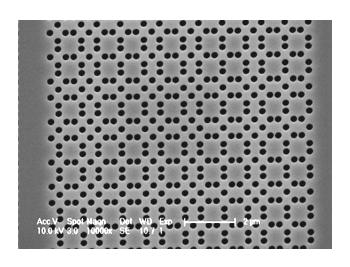
\includegraphics[width=1.6in]{chapters/2D_Thue-Morse_array_of_optical_cavities_tight-binding_model/pictures/fig1a_experimental_sem_top_view}
           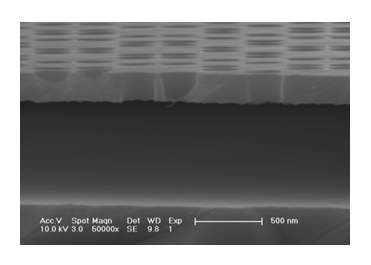
\includegraphics[width=1.75in]{chapters/2D_Thue-Morse_array_of_optical_cavities_tight-binding_model/pictures/fig1b_experimental_sem_side_view}}
\caption[Top-view SEM image of a 2D Thue-Morse array of air holes in the GaAs membrane.]{\label{fig:experimental_structure}
Left: top-view SEM image of a 2D Thue-Morse array of air holes in the GaAs membrane. Right: tilt-view SEM image of a cleaved sample showing the perforated GaAs membrane free standing in air. White scale bars from left to right are 2$\mu$m and 500nm.}
\end{figure}

The 2D Thue-Morse pattern is usually constructed in two steps~\cite{2008_Negro}. First, the 1D Thue-Morse sequence is generated by starting with letter~$A$ (generation $g=0$) and repeatedly applying the inflation rules $A\rightarrow AB$ and $B\rightarrow BA$. After $g$ iterations the number of elements in the binary sequence is~$2^g$. The complimentary system is obtained by simultaneous replacements of $A\rightarrow B$ and $B\rightarrow A$. In the second step, using the~$2^g$ elements of the 1D sequence obtained previously as seeds, we build 1D Thue-Morse sequences of $g$'th generation along the second dimension of the structure. $A$~elements in the resulting~$2^g\times2^g$ array define the position of the ``particles,'' such as e.g. cylindrical holes in a dielectric membrane, c.f. Fig.~\ref{fig:experimental_structure}. 

Figure~\ref{fig:ThMo_reduction}(a) depicts the 2D Thue-Morse structure with $g=6$ obtained using the above procedure. We observe the occurrence of clusters formed at the places of missing $2\times2$ holes. Holes surrounding a cavity in the dielectric membrane~\cite{2011_Cao_DAS} create a mismatch in the effective refractive index between the inside and outside regions. Hence, in certain spectral ranges the cluster regions can support cavity modes and thus play an important role in determining transport properties of the system~\cite{2007_Moretti,2008_Boriskina,2011_Cao_DAS}. In the structure shown in Fig.~\ref{fig:ThMo_reduction}(a), however, a number of modes exist that are not directly associated with the $2\times2$ clusters. This is because (i) the structure contains other ($2\times 1$ and $1\times 1$) voids, and (ii) the $2\times 2$ clusters can occur in corner-sharing arrangements. The latter can cause strong hybridization due to excessive coupling.

With the goal of obtaining a 2D~DAS amenable to tight-binding description hereafter we propose to use a Thue-Morse-based array of micro-cavities constructed as follows. First, in the original Thue-Morse array shown in Fig.~\ref{fig:ThMo_reduction}(a) we retain only $2\times2$ clusters as shown in Fig.~\ref{fig:ThMo_reduction}(c). Second, to avoid occurrence of multiple modes we reduce the size of the clusters from $2\times2$ to obtain $1\times1$ micro-cavities. In addition, we insert an extra row/column between the adjacent cavities to prevent excessive inter-cavity coupling. The obtained array of micro-cavities, shown in Fig.~\ref{fig:ThMo_reduction}(e), has a similar spatial Fourier spectrum when compared with the original Thue-Morse structure, thus retaining the structural characteristics of the DAS, c.f. Fig.~\ref{fig:ThMo_reduction}(b,d,f). 

\begin{figure}%[t]
\vskip -0.1in
\centering{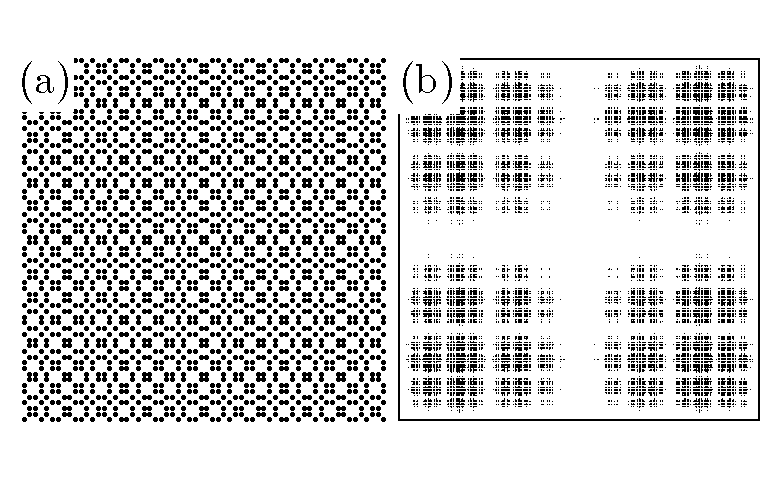
\includegraphics[width=4in]{chapters/2D_Thue-Morse_array_of_optical_cavities_tight-binding_model/pictures/fig2ab_Thue-Morse_MediumGen6_FT8_compliment0_scatSize1}}
\vskip -0.1in
\centering{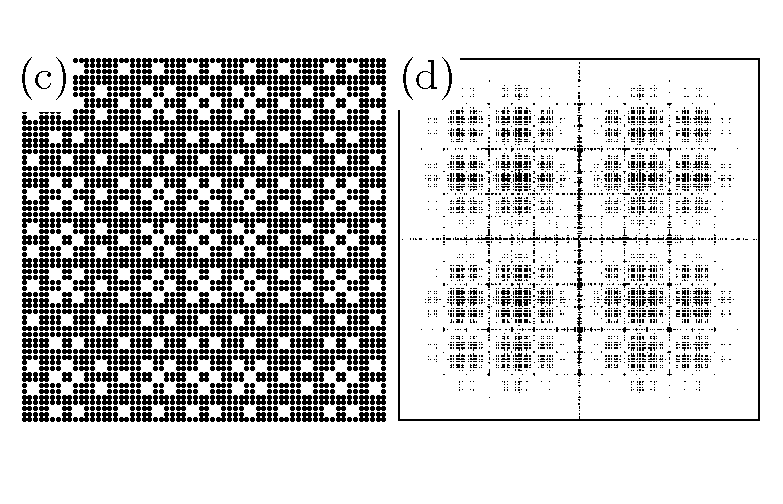
\includegraphics[width=4in]{chapters/2D_Thue-Morse_array_of_optical_cavities_tight-binding_model/pictures/fig2cd_Thue-Morse_cavities_only_MediumGen6_FT8_compliment1_scatSize1}}
\vskip -0.1in
\centering{\includegraphics[width=4in]{chapters/2D_Thue-Morse_array_of_optical_cavities_tight-binding_model/pictures/fig2ef_Comsol_Thue-Morse_MediumGen6_FT8_compliment1_scatSize1}}
\vskip -0.1in
\caption[Construction of Thue-Morse based array of micro-cavities.]{\label{fig:ThMo_reduction} Construction of Thue-Morse based array of micro-cavities. First, all $1\times1$ and $2\times1$ voids in the original 2D Thue-Morse structure are filled to obtain (c). Then $2\times2$ clusters are reduced to $1\times1$ and separated by an additional row/column of holes (e). (b,d,f) show the spatial Fourier spectra of the structures shown in (a,c,e), respectively.}
\end{figure}

We use finite difference frequency domain (FDFD) calculations in the commercial package Comsol to calculate the resonant mode in an uncoupled cavity formed by one missing hole in a square lattice, and verify that it indeed supports only one tightly confined mode with an eigenfrequency inside the photonic bandgap of the underlying square lattice, c.f.~Fig.~\ref{fig:comsol_model}(a), with the ratio between radius of the hole and the lattice spacing $r/a=0.35$. The photonic band structures of the 2D square lattice can be computed with the readily available simulation package MPB~\cite{2001_Johnson_Joannopoulos_mpb}. The effective refractive index $n_{eff}=2.7$ of 2D structure is found by comparing 3D bandgap calculations of the experimentally realized GaAs membrane in Fig.~\ref{fig:experimental_structure} with thickness $t=400nm$; wavelength is assumed to be $\lambda=800nm$. 

To provide further support of applicability of the tight-binding description we found all eigenstates in a portion of Thue-Morse based DAS in Fig.~\ref{fig:ThMo_reduction}(e) containing forty micro-cavities. As an example, one of exactly forty eigenstates is shown in Fig.~\ref{fig:comsol_model}(b) demonstrating that it is indeed a superposition of the modes of the individual cavities. Moreover, we find that frequencies of all eigenstates lie inside the photonic gap of the underlying square lattice. In the next section we will employ the tight-binding approximation to study the spatial confinement of these eigenstates.

\begin{figure}%[h]
\vskip -0.15in
\centering{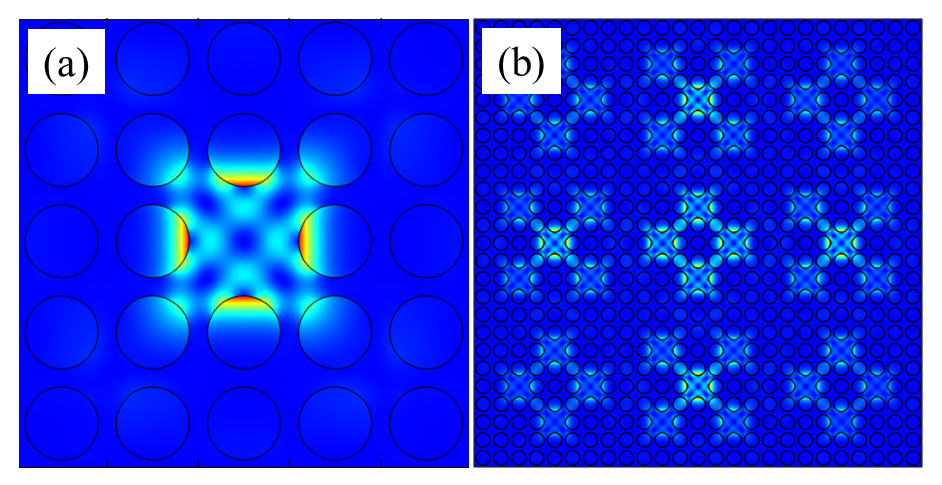
\includegraphics[width=3.5in]{chapters/2D_Thue-Morse_array_of_optical_cavities_tight-binding_model/pictures/fig3ab_comsol_model_ab}}
%\vskip -0.15in
\caption[(a) Cavity mode used as the basis in the tight-binding description of the Thue-Morse optical cavity array structure shown in Fig.~\ref{fig:ThMo_reduction}(e).]{\label{fig:comsol_model} (a) Cavity mode used as the basis in the tight-binding description of the Thue-Morse optical cavity array structure shown in Fig.~\ref{fig:ThMo_reduction}(e). (b) shows an example of an eigenmode computed by Comsol FDFD simulations with closed boundary conditions. The eigenmode is composed of the hybridized modes of the individual cavities.}
\end{figure}

%FAILURE IN ps2pdf
\section{Tight binding analysis}
% \ \\
% \addcontentsline{toc}{section}{1.3\ \ \ Tight-Binding Analysis}\noindent\textbf{1.3 TIGHT-BINDING ANALYSIS}
\label{sec:tb}

The tight-binding model~\cite{1954_Slater_tightBinding} has been a powerful tool in studies of DAS~\cite{2009_Barber}. The Thue-Morse pattern has been studied in the framework of the tight-binding approach in 1D, where neighbors are clearly defined~\cite{1995_Carpena}. As we have shown in the previous section, a purposefully designed 2D photonic Thue-Morse system can be described in the basis of individual cavity modes. Next, we investigate the pattern of inter-cavity coupling in this aperiodic structure.

\begin{figure}%[h]
\centering{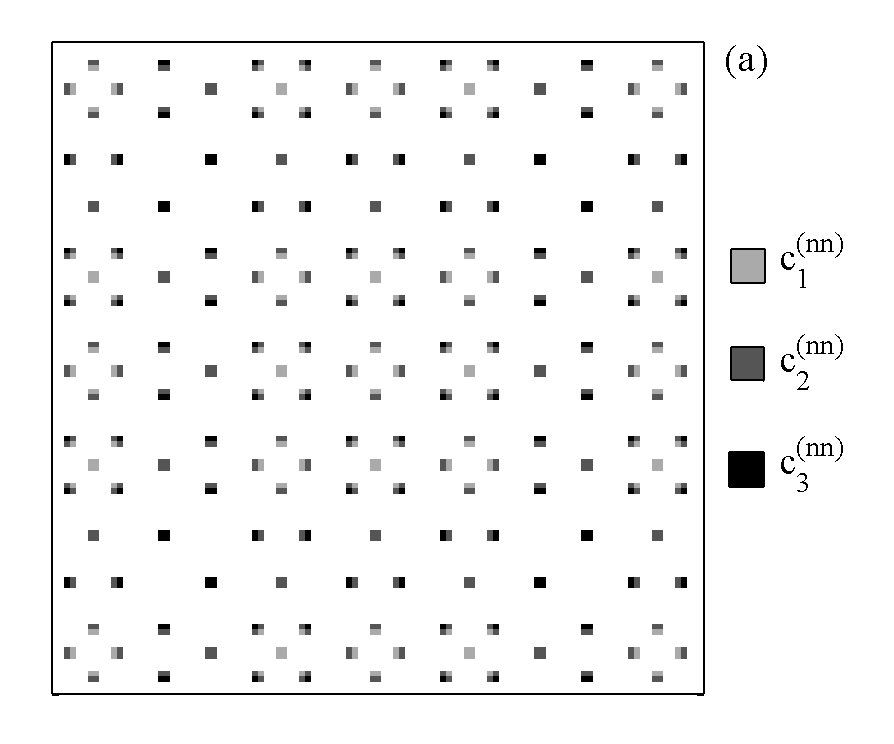
\includegraphics[width=3.5in]{chapters/2D_Thue-Morse_array_of_optical_cavities_tight-binding_model/pictures/fig4a_nn_expanded}}
\centering{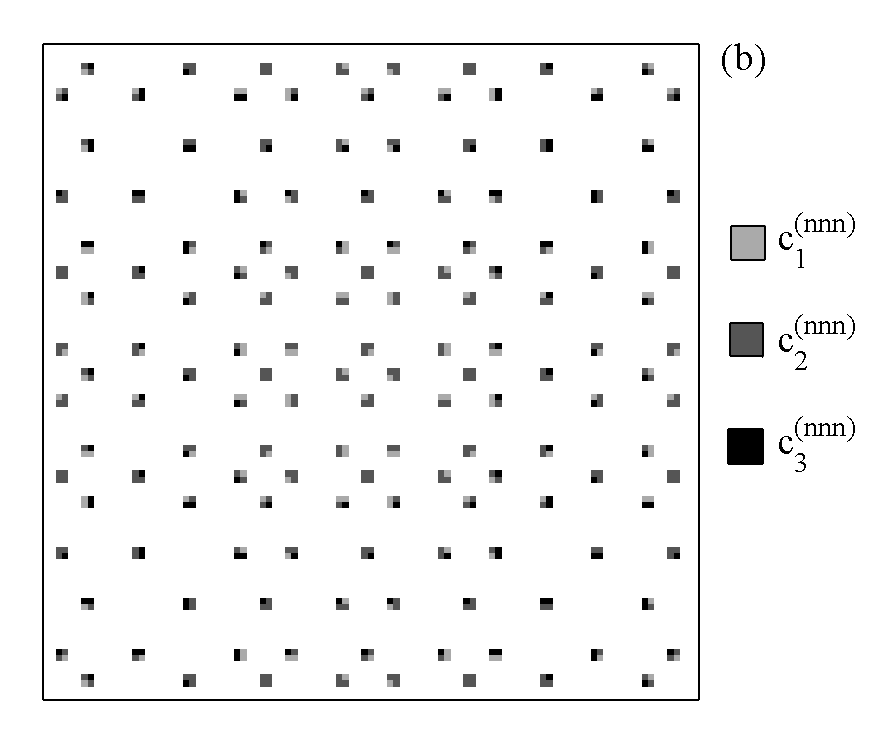
\includegraphics[width=3.5in]{chapters/2D_Thue-Morse_array_of_optical_cavities_tight-binding_model/pictures/fig4b_nnn_expanded}}
\caption[Squares at the location of each micro-cavity have four colored corners.]{\label{fig:coupling} Squares at the location of each micro-cavity have four colored corners. The color of a corner specifies one of three possible the kinds of nearest (a) and next-nearest (b) coupling in Thue-Morse based array ($g=6$) from Fig.~\ref{fig:ThMo_reduction}(e). Because we have established applicability mapping between this structure and a square lattice, there are always four nearest and four next-nearest neighbors. }
\end{figure}

Recently, in Ref.~\citenum{2012_Payne_Mapping_2D_TM} we demonstrated the possibility of mapping the array of $2\times2$ clusters, c.f. Fig.~\ref{fig:ThMo_reduction}(c), in 2D Thue-Morse DAS onto a periodic square lattice where we can use a pair of indices $i$ and $j$ to uniquely enumerate each micro-cavity.  Such mapping allowed us to  identify all configurations of nearest and next-nearest neighbors. We found that only three configurations of each type exist. Thus, the mapping reduces the original aperiodic structure to the periodic structure with aperiodic arrangement of the limited set of pairings. Because the structure considered in this work, c.f.~Fig.~\ref{fig:ThMo_reduction}(e), is isomorphic to that shown in Fig.~\ref{fig:ThMo_reduction}(a), the mapping procedure can also be performed here. Figures~\ref{fig:coupling}(a,b) show the patterns of the nearest $c^{(nn)}_{1-3}$ and next-nearest neighbor $c^{(nnn)}_{1-3}$  couplings, respectively. The numerical values of the pairwise coupling coefficients are found from 2D Comsol simulations. Eigenfrequencies of a two cavity system are the solutions of
\begin{equation}
\det\left(\begin{array}{cc}\omega_0&c\\ c&\omega_0\end{array}\right)=0,
\label{eq:c}
\end{equation}
which yields $\omega_\pm=\omega_0\pm c$. Thus, the frequency splitting between two eigenstates in Comsol simulations give directly $2c$. Numerical values describing the experimental system of Ref.~\citenum{2011_Cao_DAS} are listed in Table~\ref{tab:c}. Out of six possible couplings only three appear to be important including one next-nearest coupling. The latter corresponds to coupling between the diagonal cavities in the diamond arrangement in Fig.~\ref{fig:ThMo_reduction}(e).

\begin{table}
\begin{center}
\caption{\label{tab:c}Coupling coefficients for nearest and next-nearest pairings}
\begin{tabular}{||c|c|c||c|c|c||}
\hline
$c^{(nn)}_{1}$ & $c^{(nn)}_{2}$ & $c^{(nn)}_{3}$ & $c^{(nnn)}_{1}$ & $c^{(nnn)}_{2}$ & $c^{(nnn)}_{3}$ \\ \hline
$0.004105$ & $0.000915$ & $0.000238$ & $0.002034$ & $0.000736$ & $0.000261$ \\
% from /svn/research/Project_DAS/2012_TB_for_2DTM_manuscript/TB_for_2DTM.xlsx SVN 3082
\hline
\end{tabular}
\end{center}

\ \\
Coupling coefficients, c.f.~Fig.~\ref{fig:coupling}, in the tight-binding description of the system shown in Fig.~\ref{fig:ThMo_reduction}(e). Numerical values are found from Eq.~(\ref{eq:c}) in 2D Comsol simulation of the structure with $n_{eff}=2.7$, $r/a=0.35$. $\omega_0$ is found to be $2\pi/a\times0.3266$.
\end{table}

Hybridization of the modes of individual micro-cavities is obtained by the diagonalization of the tight-binding Hamiltonian
\begin{equation}
\omega_0\ \psi_{ij}+\sum_{i^\prime j^\prime}c_{ij,i^\prime j^\prime}\ \psi_{i^\prime j^\prime}=\omega\psi_{ij},
\label{eq:TB_hamiltonian}
\end{equation}
where $\omega_0$ is the energy of the stand-alone cavity, $\psi_{ij}$ is the field amplitude of the $ij$'th cavity. Here the indexes $i$ and $j$ enumerate the cavities based on the mapping procedure in Ref.~\citenum{2012_Payne_Mapping_2D_TM}. Furthermore, $c_{ij,i^\prime j^\prime}$ denotes the coupling coefficient between the cavities located at $ij$ and $i^\prime j^\prime$. Based on the analysis of physical proximity in the Thue-Morse structure, c.f.~Fig.~\ref{fig:ThMo_reduction}(e), we limit the consideration to two types of coupling -- nearest ($i^\prime=i\pm1$ and $j^\prime=j$, or $i^\prime=i$ and $j^\prime=j\pm1$) and next-nearest ($i^\prime=i\pm1$ and $j^\prime=j\pm1$) couplings only. As discussed above, $c_{ij,i^\prime j^\prime}$ can take one of only six possible values, three of each type, c.f.~Fig.~\ref{fig:coupling}. Therefore, the structural complexity in the arrangement of cavities in the original structure has been reduced to the complexity in connectivities between the elements of the ordered array in Eq.~(\ref{eq:TB_hamiltonian}). 

\begin{figure}%[h]
\vskip -0.15in
\centering{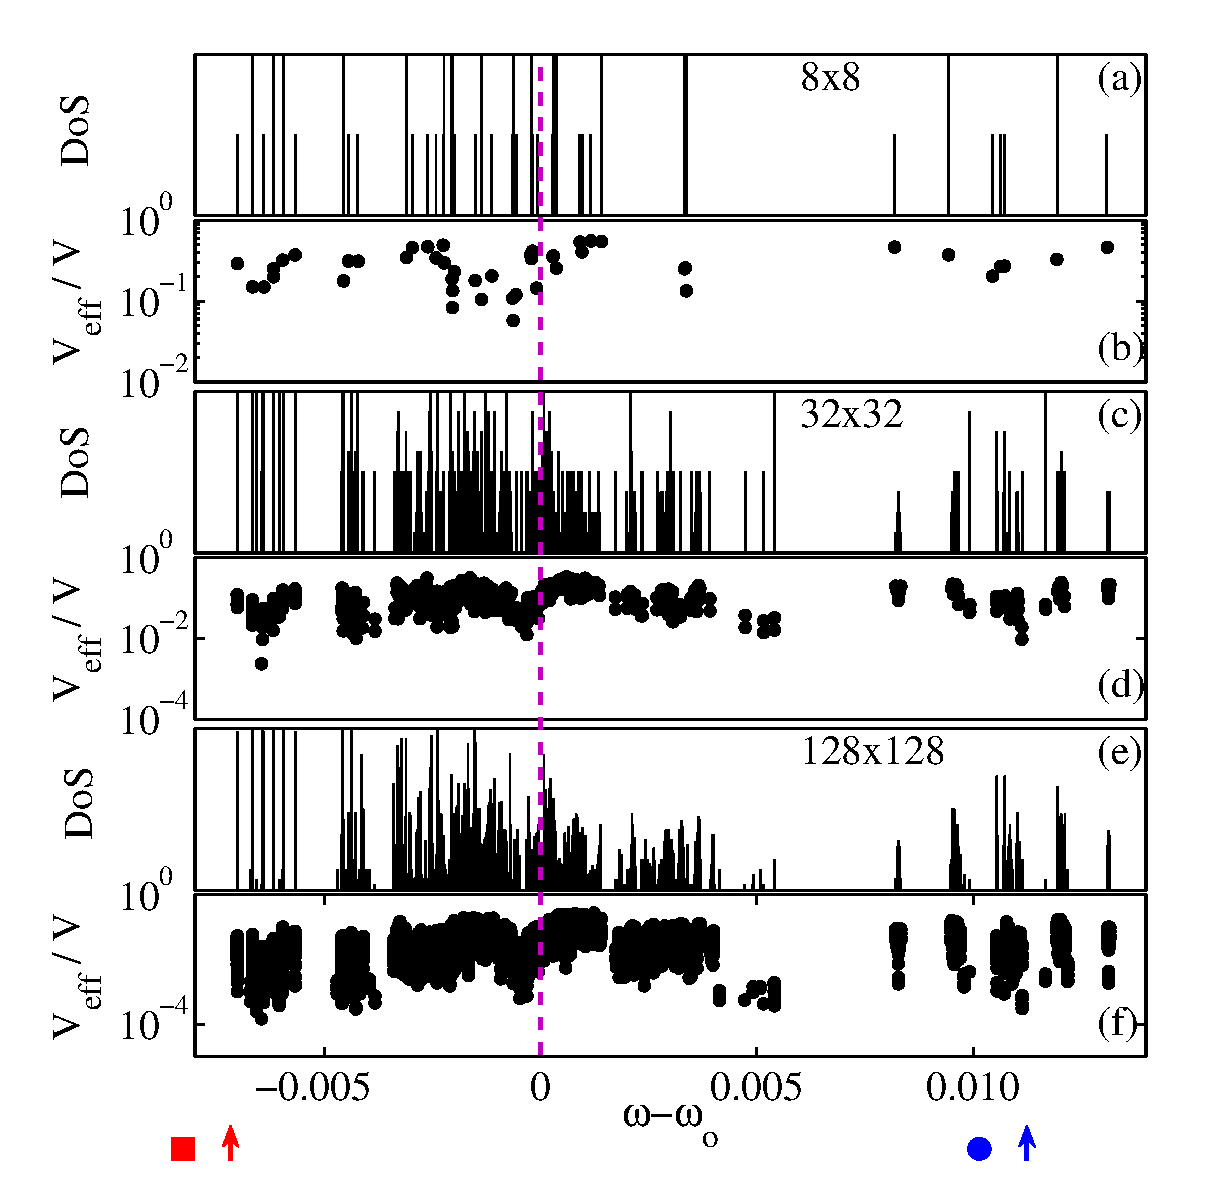
\includegraphics[width=5in]{chapters/2D_Thue-Morse_array_of_optical_cavities_tight-binding_model/pictures/fig5_IPR_N8_32_128_log_with_DoS}}
\vskip -0.15in
\caption[Density of states (a,c,e) and the inverse participation ratio (b,d,f) are computed from Eqs.~(\ref{eq:dos},\ref{eq:IPR}) for $N\times N$ 2D Thue-Morse based arrays of optical micro-cavities in Fig.~\ref{fig:ThMo_reduction}(e) in the framework of the 2D tight-binding model defined by Eq.~(\ref{eq:TB_hamiltonian}).]{\label{fig:tm_dos} Density of states (a,c,e) and the inverse participation ratio (b,d,f) are computed from Eqs.~(\ref{eq:dos},\ref{eq:IPR}) for $N\times N$ 2D Thue-Morse based arrays of optical micro-cavities in Fig.~\ref{fig:ThMo_reduction}(e) in the framework of the 2D tight-binding model defined by Eq.~(\ref{eq:TB_hamiltonian}). Nearest and next-nearest neighbor couplings in Figs~\ref{fig:coupling}(a,b) and Table~\ref{tab:c} are extracted from FDFD Comsol simulations of the experimental system in Ref.~\citenum{2011_Cao_DAS}. The complex structure of the spectrum emerges with an increase of $N$ with extended ($V_{eff}(\omega^{(m)})/V\sim 1$) and localized ($V_{eff}(\omega^{(m)})/V\ll 1$) states coexisting in very narrow frequency windows. }
\end{figure}

Having found the pattern of inter-cavity couplings we now analyze the spectrum of eigenfrequencies $\omega^{(m)}$ and the corresponding eigenstates $\psi^{(m)}_{ij}$ in Eq.~(\ref{eq:TB_hamiltonian}). Importantly, our tight binding analysis enables thorough theoretical investigations of e.g. hierarchical structure, existence of multiple length scales, and their effects on localization in DAS. Fig.~\ref{fig:tm_dos} shows the optical density of states (DoS) defined as
\begin{equation}
DoS(\omega)=\sum_n\delta(\omega-\omega^{(m)}).
\label{eq:dos}
\end{equation}
It exhibits complex structure with dense sets of {\it coexisting} confined and extended states. This can be directly witnessed by computing the inverse participation ratio (IPR)
\begin{equation}
IPR(\omega^{(m)})\equiv\frac{V_{eff}(\omega^{(m)})}{V}=\left[\frac{V\times\sum_{ij}\left|\psi^{(m)}_{ij}\right|^4}{\left(\sum_{ij}\left|\psi^{(m)}_{ij}\right|^2\right)^2}\right]^{-1}, 
\label{eq:IPR}
\end{equation}
where $V_{eff}(\omega^{(m)})/V$ defines the fraction of the total (2D) volume occupied by the eigenstate $\psi^{(m)}_{ij}$. Figs.~\ref{fig:tm_dos}(b,d,f) demonstrate that, while some states become progressively more localized as the size of the system increases, the others remain extended: $V_{eff}(\omega^{(m)})/V\sim1$. Furthermore, the spatial profiles of some of the extended states maintain a nearly constant intensity distribution across the entire structure, c.f. Fig.~\ref{fig:state_profiles}. 

\begin{figure}%[h]
\vskip -0.15in
\centering{\includegraphics[width=3.5in]{chapters/2D_Thue-Morse_array_of_optical_cavities_tight-binding_model/pictures/fig6_TB_TM_eigenstate_profile_sizeCavityArray40_localized_extended}}
\vskip -0.15in
\caption[Extended (nearly-constant throughout the entire volume, blue circles) and localized (red squares) eigenstates supported by $40\times 40$ 2D Thue-Morse based array of optical micro-cavities.]{\label{fig:state_profiles} %[Color online.] 
Extended (nearly-constant throughout the entire volume, red squares) and localized (blue circles) eigenstates supported by $40\times 40$ 2D Thue-Morse based array of optical micro-cavities. Arrows and circle,square at bottom of Fig.~\ref{fig:tm_dos} indicate the location of these eigenstates.}
\end{figure}

\section{Conclusions}
% \ \\
% \addcontentsline{toc}{section}{1.4\ \ \ CONCLUSIONS}\noindent\textbf{1.4 CONCLUSIONS}
\label{sec:conclusions_TB}
% \\*
In this work we demonstrated the applicability of the tight binding approach in a deterministic aperiodic array of photonic micro-cavities. Using an isomorphic mapping, complex structural correlations characteristic of the Thue-Morse sequence with singular-continuous spatial Fourier transform were replaced with aperiodic couplings in a square lattice. Under realistic conditions, we observed hybridization of the modes of individual micro-cavities into the eigenstates of the entire array. Our work adds the tight binding approach to the arsenal of theoretical tools for studying of 2D~Thue-Morse structures as well as for design and analysis of experiments.

Results obtained above with the tight-binding model further reinforce the conclusions reached in previous works about anomalous optical transport properties in Thue-Morse DAS. The tight binding model allows us to investigate the size scaling of the density of the optical states in large $N\times N$ arrays of optical micro-cavities; monitor the evolution of the spectra; and to study spatial properties of the eigenstates via e.g. the inverse participation ratio. The tight-binding model allows us to consider very large 2D~DAS to obtain general (model-independent) results. Realistic systems, such as those in Ref.~\citenum{2011_Cao_DAS}, with the size of up to $150\mu m\times 150\mu m$ can be studied. 

In the system considered here, the spectrum shows very peculiar hierarchical structure with photonic gaps being populated with an increase of system size. The inverse participation ratio shows coexistence of localized and extended states in the same spectral regions. Some of the extended states have nearly constant intensity across the entire sample. This property makes the considered system extremely promising for practical applications in optical control of light propagation via e.g. wave-front shaping.
 
\section{Acknowledgments} 
% \ \\
% \addcontentsline{toc}{section}{1.5\ \ \ ACKNOWLEDGMENTS}\noindent\textbf{ACKNOWLEDGMENTS}
% \\*
The authors acknowledge support by National Science Foundation Grant Nos. DMR-0704981 and DMR-0808937. LS acknowledges the support of Opportunities for Undergraduate Research Experiences at Missouri University of Science and Technology.

% % \bibliography{../../Bibliography/latex_bibliography}
% % \end{document}
